\documentclass[10pt]{article}
\usepackage[utf8x]{inputenc} 
\usepackage[english]{babel}
\usepackage{microtype}
%% erlaubt Listen einfacher zu formatieren (bietet nosep für kompakte Listen)
\usepackage{enumitem}
%% erlaubt hübsche Tabellen über mehrere Seiten, beinhaltet booktabs (\toprule, \midrule, ...)
\usepackage{ctable}
\usepackage{xcolor}
\usepackage{amsfonts,amsmath,amsthm,amssymb}
%% vordefinierte Einheiten, einfaches Angeben von Einheiten (\SI{8 \pm 1}{cm})
%%   die Unsicherheit soll mit +- abgetrennt werden
\usepackage[separate-uncertainty]{siunitx}
\sisetup{
    range-units = single,       % \SIrange soll die Einheit nur einmal anzeigen
    list-units  = repeat,       % \SIlist soll die Einheit wiederholen
}

\usepackage{graphicx}
\usepackage{float}
\usepackage{subfig}
\DeclareGraphicsExtensions{.pdf,.png,.jpg}

\usepackage{parskip}
\usepackage[final]{showkeys} \usepackage[
 a4paper,
 total={16cm,26cm},          % Breite und Höhe des Inhalt-Bereichs
 top=20mm, left=25mm,        % Ränder oben und links (war am Anfang bei left=30mm)
 headsep=10mm,               % Abstand des unteren Rands der Kopfzeile vom oberen Rand des Inhalts
 footskip=10mm               % Abstand des unteren des Inhalts zum oberen Rand der Fusszeile
]{geometry}
%% definiert \cref: Referenzen mit korrekter Bezeichnung (z.B. "Abbildung 1")
%%   die Nummer alleine ist weiter mittels \ref verfügbar
\usepackage[english, capitalise]{cleveref}


%% Angaben für \maketitle
\title{Heat of melting and evaporation of water}
\author{Hannes Imboden}
% \date{7. Mai 2013}             % ohne Angabe wird das heutig Datum verwendet

\makeatletter
%\hypersetup{
 % pdfauthor = {\@author},
  %pdftitle = {\@title},
%}
\makeatother

\begin{document}

\begin{abstract}
\noindent
The goal of this experiment was to measure the resistance of the superconductor YBa$_2$Cu$_3$O$_{7-\mathrm{\delta}}$ and to determine the transition temperature $T_c$.
\end{abstract}


\section{Introduction}
Superconductivity in metals and alloys is characterized by a sudden disappearance of resistance for temperatures lower than a certain transition temperature, $T_c$. This temperature is not the same for different materials. Some become superconducting at less than 5K (Mercury for example) while some can still be superconducting above 130K (Hg-Ba-Ca-Cu-O). \\
In our experiment, YBa$_2$Cu$_3$O$_{7-\mathrm{\delta}}$ was used. This material has a transition temperature of around 92K.

\begin{figure}[H]
\centering
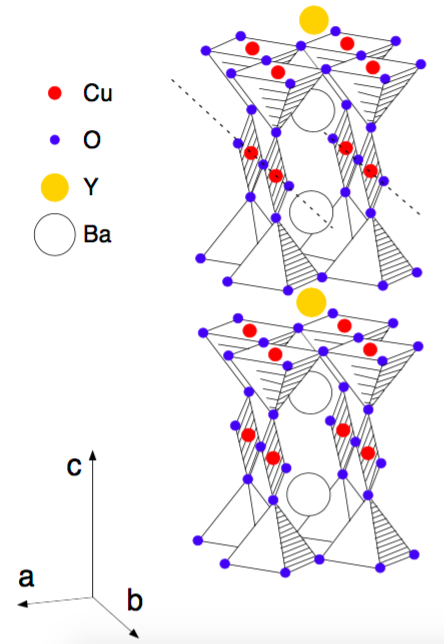
\includegraphics[width=6cm]{supercond.png}
\caption{Crystal structure of YBa$_2$Cu$_3$O$_{7-\mathrm{\delta}}$}
\end{figure}


\section{Experimental setup $\&$ Procedure}
The setup consists of four main parts:\\
\begin{itemize}
\item The specimen holder.\\
 This is where the superconductor was placed.\\ This container was equipped with connections for the temperature sensor, the heating, the resistance measurement and both current supply and voltage supply.\\
\item The cryostat.\\
This part serves to regulate the temperature. The sample is enclosed in a tube, which is submerged in liquid nitrogen. To keep the sample at a certain temperature, a heating foil is attached behind the sample. The foil will heat the sample, as more current is applied to it. This heating foil is needed, as liquid nitrogen has a constant temperature of around 77K at atmospheric pressure. \\
\item The vacuum system.\\
A vacuum of $2.8 \cdot 10^{-3}$mbar was created inside the tube. This vacuum helps to reduce the heat transfer between the probe and its surroundings, as heat is primarily exchanged through convection. With increasing vacuum, less convection can occur, as less air is inside the tube. 
\item The electromagnet.\\
The tip of the tube with the sample, including the cooling, was placed inside an electromagnet. The dependence of the resistance for different static magnetic fields could thus be measured.
\end{itemize}

~\\
  
Before measuring the resistance of our superconductor, the sample was cooled down to around 82K. The cooling (as well as the heating) was then cut out and the resistance was measured. The sample's temperature then increased slowly, as the surrounding room temperature was much higher. Thanks to the isolation created by the vacuum however, this temperature change was very slow. This allowed for a precise measurement of the transition temperature $T_c$.\\
To get the best possible measurement for the resistance, we used the so called four point measuring. The current supply is independent of the voltage metering. This allows for an undisturbed measuring of the voltage. 

\begin{figure}[H]
\centering
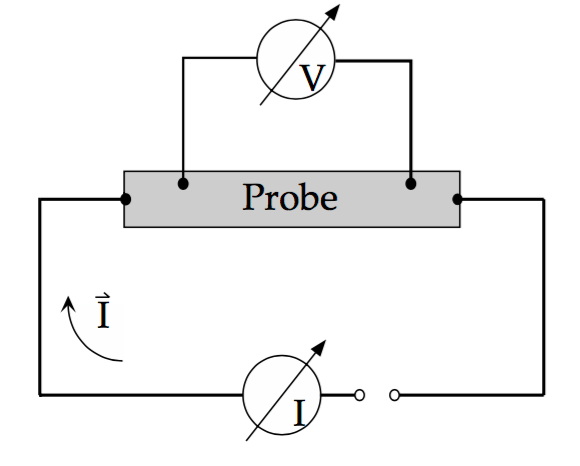
\includegraphics[width=7cm]{vierpunkt.png}
\caption{Illustration of the four-point measuring technique}
\end{figure}

















\end{document}